\begin{IEEEbiography}[{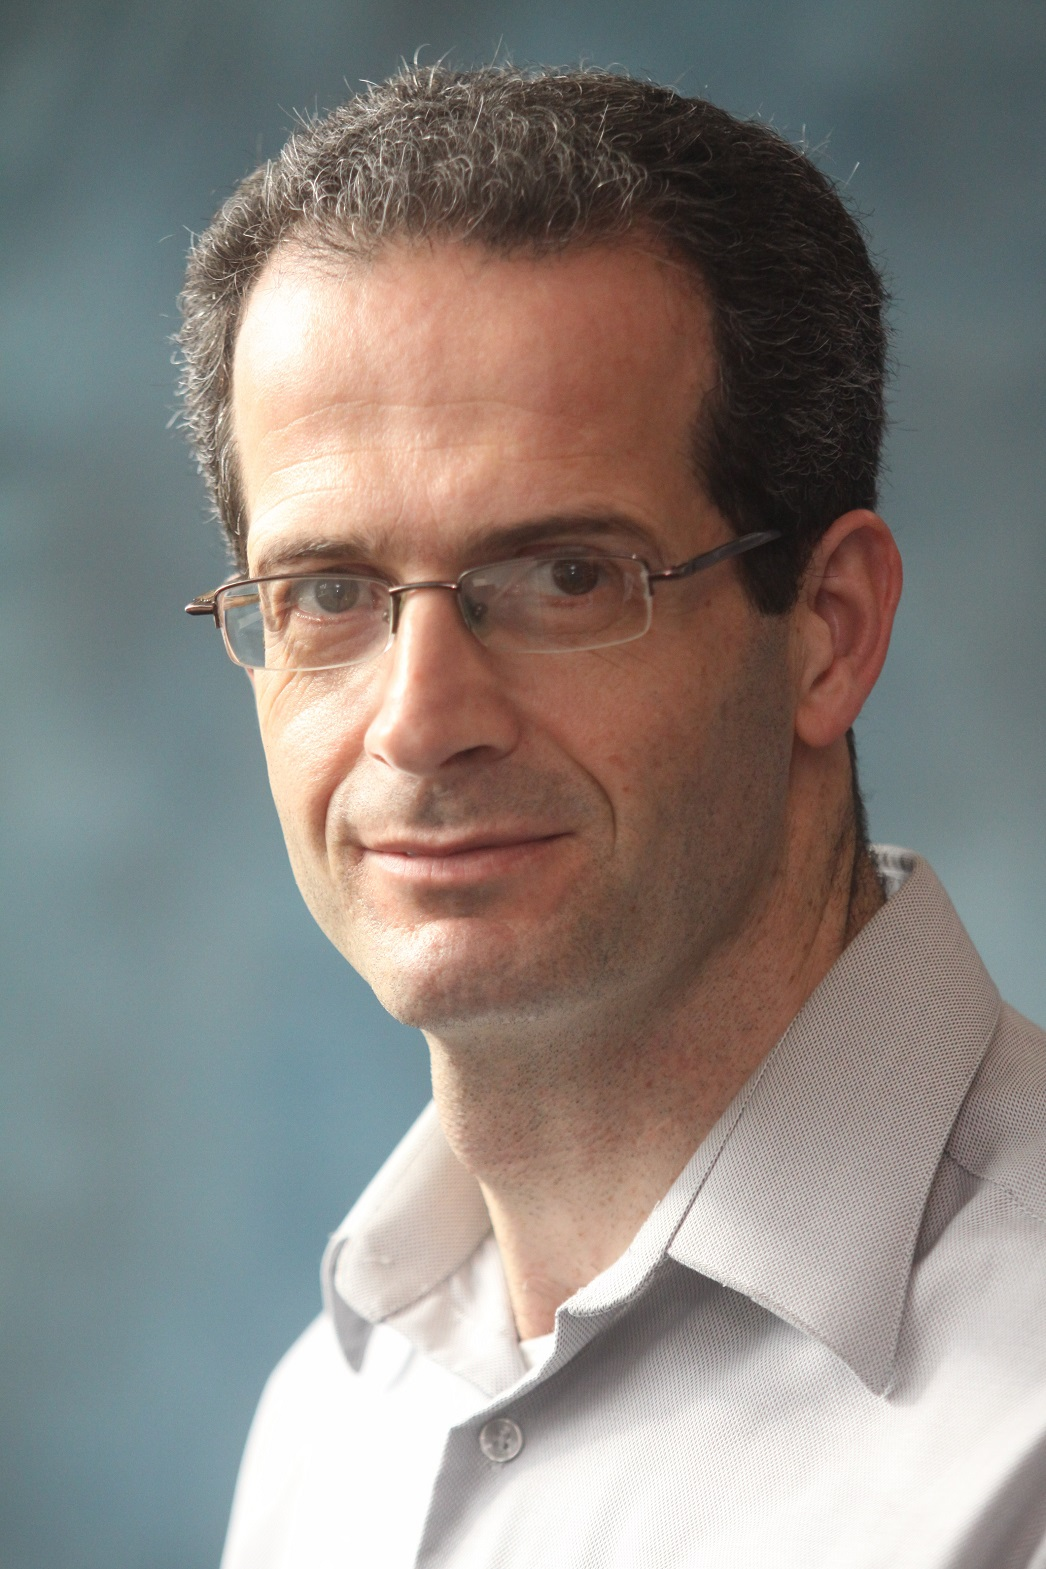
\includegraphics[width=1in,height
=1.25in,clip,keepaspectratio]{./Media/IsraelCohen.jpg}}]{Israel Cohen} (M'01-SM'03-F'15)
received the B.Sc. (Summa Cum Laude), M.Sc.
and Ph.D. degrees in electrical engineering from the Technion -- Israel Institute of
Technology, , Haifa, Israel, in 1990, 1993 and 1998, respectively.
He is currently the Louis and Samuel Seidan Professor in electrical engineering at the Technion -- Israel Institute of Technology.
He is also a Visiting Professor at Northwestern Polytechnical University, Xi’an, China.

From 1990 to 1998, he was a Research Scientist with RAFAEL Research
Laboratories, Haifa, Israel Ministry of Defense. From 1998 to 2001,
he was a Postdoctoral Research Associate with the Computer Science
Department, Yale University, New Haven, CT, USA. In 2001 he joined the
Electrical Engineering Department of the Technion.
%
He is a coeditor of the Multichannel Speech
Processing Section of the \textit{Springer Handbook of Speech
Processing} (Springer, 2008), and the coauthor of \textit{Fundamentals of Signal Enhancement and Array Signal Processing} (Wiley-IEEE Press, 2018).
%
His research interests are array processing, statistical signal processing, deep learning,
analysis and modeling of acoustic signals, speech enhancement, noise
estimation, microphone arrays, source localization, blind source
separation, system identification and adaptive filtering.

Dr. Cohen was the recipient of the Norman Seiden Prize for Academic Excellence (2017),
the SPS Signal Processing Letters Best Paper Award (2014),
the Alexander Goldberg Prize for Excellence in Research (2010),
and the Muriel and David Jacknow Award for Excellence in Teaching (2009).
He is an Associate Member of the IEEE Audio and Acoustic Signal Processing Technical Committee, and Distinguished Lecturer of the IEEE Signal Processing Society.
He was as Associate Editor of the \textsc{IEEE Transactions on Audio, Speech, and Language
Processing} and \textsc{IEEE Signal Processing Letters} and a Member of the IEEE Audio and Acoustic Signal Processing Technical Committee and the IEEE Speech and Language Processing Technical Committee.

\end{IEEEbiography}
